\chapter{Interval Graphs}

An interval graph is a graph $G$ that is the intersection graph of a collection
of closed intervals in $\mathbb{R}$. If the length of each interval is unitary,
then $G$ is a unit interval graph (UIG). UIG is equivalent to the proper interval graph, where no interval can be properly included in another one.

First we present the main characterizations of interval graphs. In the next sections we present some other subclasses of interval graphs that will help us characterize the thin strip graphs on chapter \ref{chap:thinDef}.

\begin{theorem}[Fishburn \cite{FISHBURN1985135}]
  \label{theo:intervalChord}
  $G$ is an interval graph if and only if every simple cycle of four or more
  points has a chord and any three independent vertices can be ordered ($u<v<w$) such that every path from $u$ to $w$ passes through a neighbour of $v$.
\end{theorem}

\begin{theorem}
  An interval graph is a unit interval graph if and only if it has no induced subgraph $K_{1,3}$ \cite{roberts1968representations}.
\end{theorem}

\section{Mixed Unit Interval Graphs}
\label{sec:muig}

Another interesting class of interval graphs are mixed unit interval graphs, where each
interval can be closed, open, open-closed or closed-open. In this paper we will
denote those four classes like this:

$$\mathcal{I}^{++} = \{[x,y] : x,y \in \mathbb{R}, x\leq y\}$$
$$\mathcal{I}^{--} = \{(x,y) : x,y \in \mathbb{R}, x\leq y\}$$
$$\mathcal{I}^{+-} = \{[x,y) : x,y \in \mathbb{R}, x\leq y\}$$
$$\mathcal{I}^{-+} = \{(x,y] : x,y \in \mathbb{R}, x\leq y\}$$

$\mathcal{I}$ will be replaced by $\mathcal{U}$ when we are talking about unit
mixed interval graphs and their class is denoted MUIG.

\begin{theorem}
  The classes of the graphs $\mathcal{U}^{--}$, $\mathcal{U}^{++}$,
  $\mathcal{U}^{-+}$, $\mathcal{U}^{+-}$, and  $\mathcal{U}^{-+} \cup
  \mathcal{U}^{+-}$ are the same (equivalent for $\mathcal{I}$). \cite{DOURADO20123357}
\end{theorem}

\begin{figure}
\centering
\begin{scaletikzpicturetowidth}{\textwidth}
\begin{tikzpicture}[scale=1.5]

  \draw[{(-)}] (-1,-0.5) -- (0,-0.5);
  \draw[color=black] (-0.4845,-0.8507) node {$v_4$};
  \draw[{[-}] (0,-1.5) -- (1,-1.5);
  \draw[color=black] (0.5023,-1.3568) node {$v_3$};
  \draw[{-]}] (-2,-1.5) -- (-1,-1.5);
  \draw[color=black] (-0.4899,-0.3468) node {$v_2$};
  \draw[{[-]}] (-1,-1) -- (0,-1);
  \draw[color=black] (-1.4962,-1.3536) node {$v_1$};

  \node[draw,circle,inner sep=2pt,fill,label distance=1cm] (v1) at (-4,-0.25) {};
  \draw[color=black] (-4,0) node {$v_4$};
  \node[draw,circle,inner sep=2pt,fill,label distance=1cm] (v3) at (-4,-1.25) {};
  \draw[color=black] (-4,-1.5) node {$v_2$};
  \node[draw,circle,inner sep=2pt,fill,label distance=1cm] (v2) at (-5,-1.25) {};
  \draw[color=black] (-3,-1.5) node {$v_3$};
  \node[draw,circle,inner sep=2pt,fill,label distance=1cm] (v4) at (-3,-1.25) {};
  \draw[color=black] (-5,-1.5) node {$v_1$};
  \draw  (v1) edge (v2);
  \draw  (v1) edge (v3);
  \draw  (v1) edge (v4);

\end{tikzpicture}
\end{scaletikzpicturetowidth}

\caption{Representation of $K_{1,3}$ as a MUIG.}
\label{fig:muigK13}
\end{figure}

Unlike for UIG class, $K_{1,3}$ is a MUIG as seen in figure \ref{fig:muigK13}. A complete characterization by induced forbidden subgraphs have been found independently by F. Joos \cite{shuchatUnitMixedInterval2014a} and A. Schuchat et al. \cite{joosCharacterizationMixedUnit2013}. In the next subsection the characterization of F. Joos will be reviewed by adding some remarks about graph inclusions.

\subsection{Characterization}

Joos proves in his paper the following theorem:

\begin{theorem}[Joos \cite{joosCharacterizationMixedUnit2013}]
  $G$ is a MUIG if and only if it is a $\{F\}\cup\mathcal{R}\cup\mathcal{S}\cup\mathcal{S''}\cup\mathcal{T}$-free interval graph.
\end{theorem}

We will present each family of subgraphs for
An important family of forbidden induced subgraphs in paper TSG: $\mathcal{R}$
\todo{improve introduction to this subsection}

\begin{figure}
\begin{center}
  \begin{scaletikzpicturetowidth}{\textwidth}
  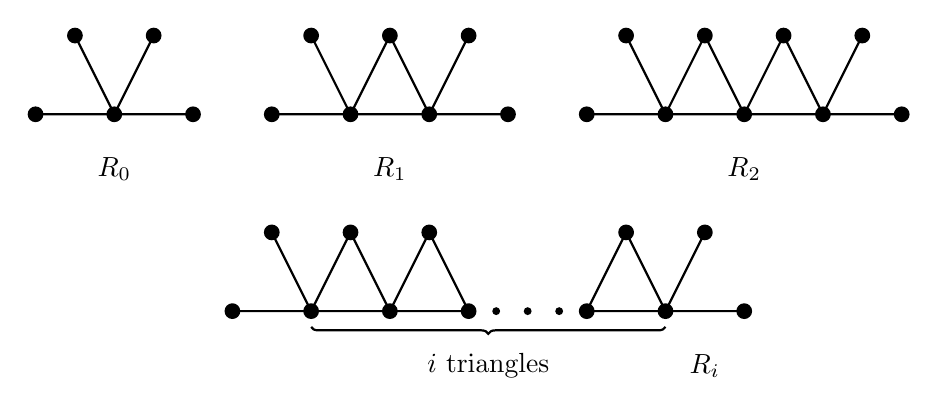
\begin{tikzpicture}[scale=1]
\def\ver{0.1} %size of a vertex
\def\x{1}

\def\xa{0.5}
\def\ya{0}

\def\xb{4}
\def\yb{0}

\def\xc{8}
\def\yc{0}

\def\xd{3.5}
\def\yd{-2.5}


%graph R_0
\path[fill] (\xa+0.5,\ya) circle (\ver);
\path[fill] (\xa+1,\ya+1) circle (\ver);
\path[fill] (\xa+2,\ya+1) circle (\ver);
\path[fill] (\xa+2.5,\ya) circle (\ver);
\path[fill] (\xa+1.5,\ya) circle (\ver);

\draw[thick] (\xa+0.5,\ya)--(\xa+1.5,\ya)--(\xa+1,\ya+1)
(\xa+2,\ya+1)--(\xa+1.5,\ya)--(\xa+2.5,\ya);

\node (1) at (\xa+1.5,\ya-0.7) {$R_0$};

%graph R_1
\path[fill] (\xb,\yb) circle (\ver);
\path[fill] (\xb+1,\yb) circle (\ver);
\path[fill] (\xb+2,\yb) circle (\ver);
\path[fill] (\xb+3,\yb) circle (\ver);
\path[fill] (\xb+0.5,\yb+1) circle (\ver);
\path[fill] (\xb+1.5,\yb+1) circle (\ver);
\path[fill] (\xb+2.5,\yb+1) circle (\ver);

\draw[thick] (\xb,\yb)--(\xb+1,\yb)--(\xb+2,\yb)--(\xb+3,\yb)
(\xb+0.5,\yb+1)--(\xb+1,\yb)--(\xb+1.5,\yb+1)--(\xb+2,\yb)--(\xb+2.5,\yb+1);

\node (1) at (\xb+1.5,\yb-0.7) {$R_1$};


%graph R_2
\path[fill] (\xc,\yc) circle (\ver);
\path[fill] (\xc+1,\yc) circle (\ver);
\path[fill] (\xc+2,\yc) circle (\ver);
\path[fill] (\xc+3,\yc) circle (\ver);
\path[fill] (\xc+4,\yc) circle (\ver);
\path[fill] (\xc+0.5,\yc+1) circle (\ver);
\path[fill] (\xc+1.5,\yc+1) circle (\ver);
\path[fill] (\xc+2.5,\yc+1) circle (\ver);
\path[fill] (\xc+3.5,\yc+1) circle (\ver);

\draw[thick] (\xc,\yc)--(\xc+1,\yc)--(\xc+2,\yc)--(\xc+3,\yc)--(\xc+4,\yc)
(\xc+0.5,\yc+1)--(\xc+1,\yc)--(\xc+1.5,\yc+1)--(\xc+2,\yc)--(\xc+2.5,\yc+1)--(\xc+3,\yc)--(\xc+3.5,\yc+1);

\node (1) at (\xc+2,\yc-0.7) {$R_2$};

%graph R_i
\path[fill] (\xd,\yd) circle (\ver);
\path[fill] (\xd+1,\yd) circle (\ver);
\path[fill] (\xd+2,\yd) circle (\ver);
\path[fill] (\xd+3,\yd) circle (\ver);
\path[fill] (\xd+4.5,\yd) circle (\ver);
\path[fill] (\xd+5.5,\yd) circle (\ver);
\path[fill] (\xd+6.5,\yd) circle (\ver);
\path[fill] (\xd+0.5,\yd+1) circle (\ver);
\path[fill] (\xd+1.5,\yd+1) circle (\ver);
\path[fill] (\xd+2.5,\yd+1) circle (\ver);
\path[fill] (\xd+5,\yd+1) circle (\ver);
\path[fill] (\xd+6,\yd+1) circle (\ver);

\fill (\xd+3.35,\yd) circle (\ver/2);
\fill (\xd+3.75,\yd) circle (\ver/2);
\fill (\xd+4.15,\yd) circle (\ver/2);

\draw[thick] (\xd,\yd)--(\xd+3,\yd)
(\xd+4.5,\yd)--(\xd+6.5,\yd)
(\xd+0.5,\yd+1)--(\xd+1,\yd)--(\xd+1.5,\yd+1)--(\xd+2,\yd)--(\xd+2.5,\yd+1)--(\xd+3,\yd)
(\xd+4.5,\yd)--(\xd+5,\yd+1)--(\xd+5.5,\yd)--(\xd+6,\yd+1);

\draw[thick,decoration={brace,mirror,raise=0.2cm},decorate] (\xd+1,\yd) -- (\xd+5.5,\yd)
node [pos=0.5,anchor=north,yshift=-0.4cm] {$i$ triangles};

\node (1) at (\xd+6,\yd-0.7) {$R_i$};

\end{tikzpicture}
\end{scaletikzpicturetowidth}
\end{center}
\caption{The class $\mathcal{R}$. \cite{joosCharacterizationMixedUnit2013}}\label{graphsR}
\end{figure}


\lemma{$\mathcal{R}$ is a family of co-comparability graphs.}
\proof{If we recall Theorem \ref{theo:spanning}, in order to prove that $\mathcal{R}$ is a family of co-comparability graphs we will have to find a spanning order for every $R_i$ with $i \geq 0$. We will proceed to label our vertices with a mapping function $f: V \to \mathbb{N}$ such that $f(v) \in [1,|V|]$. This mapping will give us a spanning order by induction:

\begin{itemize}
  \item $i = 0$: We assign the number $1$ to the vertex with maximum degree $v_1$. We assign then the rest of the numbers to the other vertices. We see then that $\forall u < v < w : uw\in E \to uv \in E$ because every vertex is adjacent to $v_1$.

  \item $i = i+1$: We define $\lambda_i = 5+2i$ where $\lambda_i = |V(R_i)|$ (the size of the graph). We have two on each graph, where their labels are $\lambda_i+1$ and $\lambda_i+2$ and there are three new edges: $v_{\lambda_i}v_{\lambda_i-1},v_{\lambda_i}v_{\lambda_i+1},v_{\lambda_i}v_{\lambda_i+2} \in E$.

  By induction we only have to see if it holds with the new edges. We can say that it still holds with $v_{\lambda_i}v_{\lambda_i-1}$ and $v_{\lambda_i}v_{\lambda_i+1}$ because:

  $$\nexists k \in \mathbb{N} : i < k < i+1$$

  Finally, we see that $v_{\lambda_i}v_{\lambda_i+2}$ is a valid edge because $v_{\lambda_i}v_{\lambda_i+1}\in E$. \qed
\end{itemize}
}

\section{Unfettered Unit Interval Graphs}

\todo[inline]{Try to characterize with known forbidden families of subgraphs (from MUIG? and TSG article)}
